% mms-euler.tex

\section{Method of manufactured solutions -- Euler flow}
\label{mms-euler-sec}
\index{source terms!user defined!example of use}\index{verification}
%
The method of manufactured solutions as a code verification exercise for inviscid flow.
This shows a sophisticated use of the user-defined source terms to
add the extra pieces required to model a known (manufactured) flow solution.

\begin{figure}[htbp]
\begin{center}
\mbox{
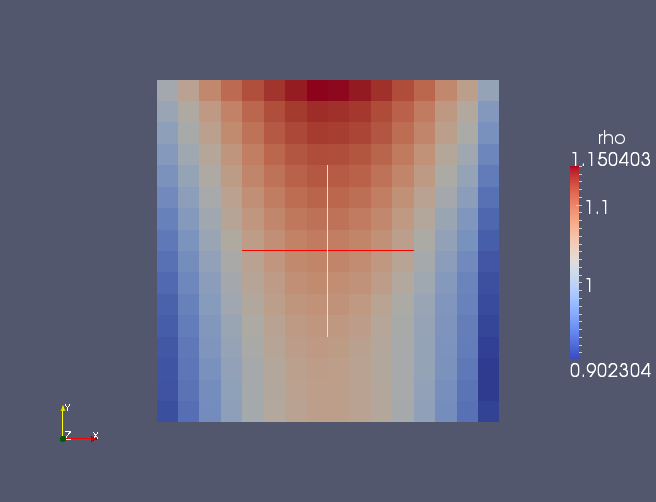
\includegraphics[width=0.5\textwidth]{../2D/mms_euler/mms-density.png}
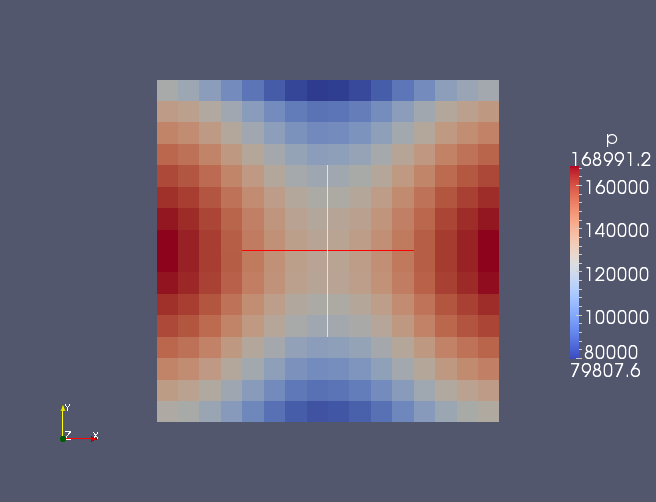
\includegraphics[width=0.5\textwidth]{../2D/mms_euler/mms-pressure.png}
}
\end{center}
\caption{Density and pressure fields for the steady-state solution for the
  Method of Manufactured Solutions.}
\label{mms-euler-density-pressure-fig}
\end{figure}


\newpage

\subsection{Input script (.py)}\index{boundary conditions!UserDefinedBC!example of use}
\topbar
\lstinputlisting[language={}]{../2D/mms_euler/euler_manufactured.py}
\bottombar

\subsection{Boundary condition file (.lua)}
\topbar
\lstinputlisting[language={}]{../2D/mms_euler/udf-bc.lua}
\bottombar

\subsection{Source term file (.lua)}
%
The source terms were generated with the aid of the Maxima computer algebra system.
\topbar
\lstinputlisting[language={}]{../2D/mms_euler/udf-source.lua}
\bottombar

\subsection{Shell scripts}
\label{mms-euler-sh-files}
\topbar
\lstinputlisting[language={}]{../2D/mms_euler/prep_simulation.sh}
\bottombar

\noindent
\topbar
\lstinputlisting[language={}]{../2D/mms_euler/run_simulation.sh}
\bottombar

\noindent
The postprocessing script shows features of the post-processor that allow
one to compare one solution with another (in order to check convergence to steady state)
and also to report the norms of the differences between the computed solution and 
a reference solution described by a Python file.
\index{e3post.py!reference function}\index{e3post.py!report norms}

\noindent
\topbar
\lstinputlisting[language={}]{../2D/mms_euler/post_simulation.sh}
\bottombar

\subsection{Python reference-function files}
\topbar
\lstinputlisting[language={}]{../2D/mms_euler/euler_verify.py}
\bottombar

\noindent
\topbar
\lstinputlisting[language={}]{../2D/mms_euler/euler_wrapper.py}
\bottombar

\subsection{Notes}
\begin{itemize}
\item This simulation required 1\,min, 18\,sec on a single core of 
  a Pentium 1.6\,GHz processor to reach a final time of 20\,ms in 1092 steps.
\end{itemize}
